\section{Resultados}
%Deben incluir los resultados de los experimentos, utilizando el formato más adecuado
%para su presentación. Deberón especificar claramente a qué experiencia corresponde
%cada resultado. No se incluirán aquí corridas de máquina. Algo fundamental en su
%aprendizaje en la materia es la presentación de resultados de forma clara y concisa para
%el lector.


\begin{figure}[H]{}
\centering
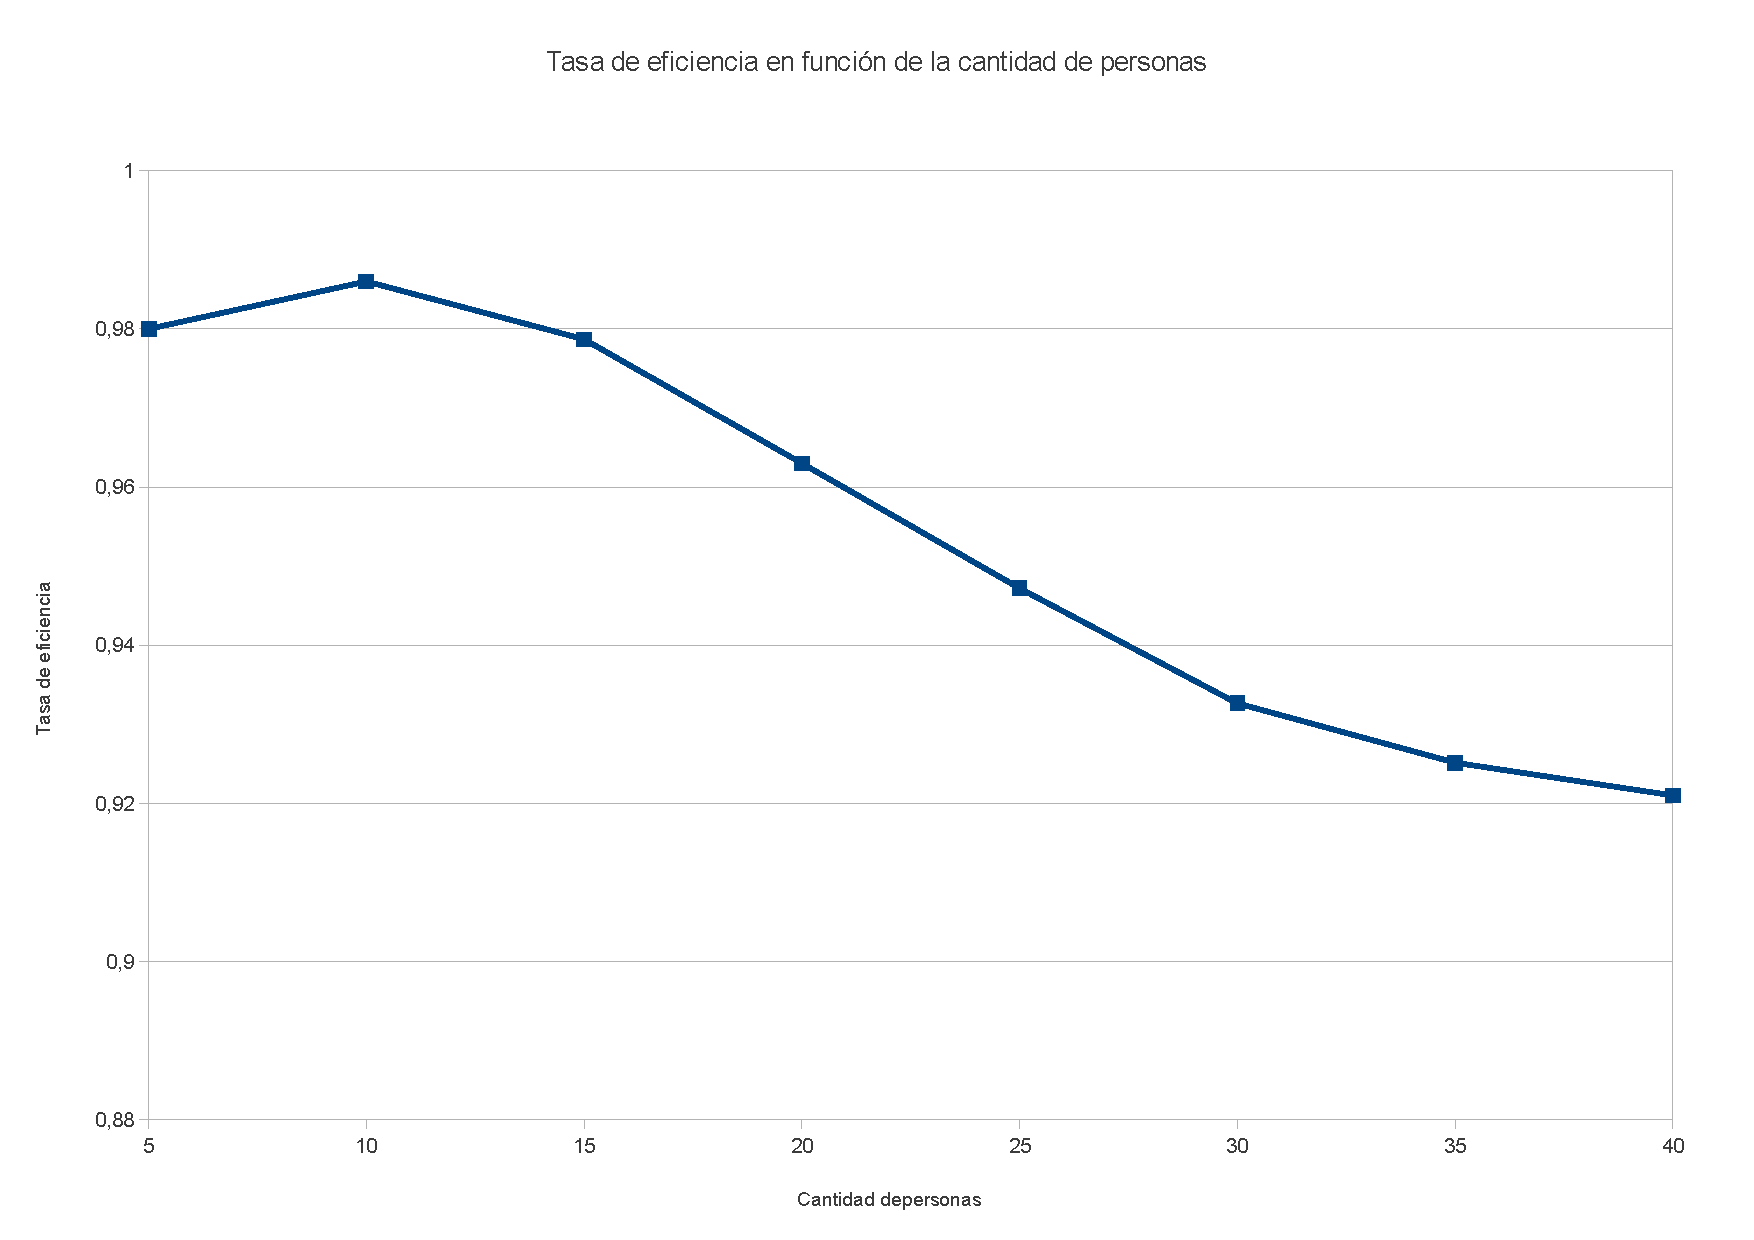
\includegraphics[scale=0.5]{graphs/CPvsTE.pdf}
\caption{Tasa de eficiencia en función de la cantidad de personas.}
\label{CPvsTE}
\end{figure}

